\documentclass{article}
\usepackage[utf8]{inputenc}
\usepackage{bm}
\usepackage{amsfonts}







\usepackage{graphicx}
\graphicspath{ {/} }






\RequirePackage[dvipsnames]{xcolor}
\RequirePackage{amsfonts}

%%This parts handles the options passed to the package.

    %\DeclareOption{red}{\renewcommand{\wordcolour}{sharelatexcolour}}
    %\DeclareOption{blue}{\renewcommand{\wordcolour}{mybluecolour}}
    %\DeclareOption*{\PackageWarning{examplepackage}{Unknown ‘\CurrentOption’}}
    %\ProcessOptions\relax

%%Body of the package, most of the declarations appear here.


\newcommand{\comment}[1]{}%define a new command that effectively does nothing with the input

\newcommand{\bigO}[1]{\mathcal{O}(#1)} %define the bigO symbol

\newcommand{\questRef}[1]{\textcolor{ForestGreen}{{\textbf{($#1_?$)}}}} %creates a question reference
\newcommand{\titem}[1]{\item{}\textit{#1}} %creates a titled item, has an argument for title 
\newcommand{\bitem}[1]{\item{}\textbf{#1}}

%number systems

\newcommand{\reals}{$\mathbb{R}$}
\newcommand{\rats}{$\mathbb{Q}$}
\newcommand{\ints}{$\mathbb{Z}$}
\newcommand{\naturals}{$\mathbb{N}$}

\newcommand{\defRef}[1]{\textcolor{Purple}{{\textbf{($#1_D$)}}}} %creates a question reference
%%Important words are added to the index and printed in different colour

%Need to add:%
% std def of DFA
% std def of a turing machine


\title{Solving Problem 47 with TMs}
\author{Matan Shtepel}
\date{August 13, 2021}

\newcommand{\K}{$\bm{K}$}
\newcommand{\aaa}{algorithm/automaton}


\begin{document}


\maketitle

\section{Relevant Definitions}
\begin{itemize}
    \titem{Problem 25:} "Axiomatically describe classes \K{} of algorithms or automata in which any algorithm/automaton has a totalling."
    \titem{Problem 26:} "Axiomatically describe classes \K{} of algorithms or automata in which any partial algorithm/automaton has an extension." Note this problem, as far as I can tell, is equivalent to problem 25, just stated from a different perspective. 
    \titem{Definabillity Problem $R_d$:} "Find an algorithm/automaton $H$ that for an arbitrary algorithm/automaton $A$ from \K{} and an arbitrary element $x$ from $D^*(K)$, informs whether $A(x)$ is defined."
    \titem{Total definition:} An algo/automata A is called total $\iff$ $DD(A)=AD(A)$.
    \titem{Partial definition:} An algo/automata A is called partial $\iff$ $DD(A)\neq{}AD(A)$
    \titem{$AD$ vs $DD$:} $AD(A)$ is the acceptability domain, all the inputs $A$ can accept. $DD(A)$ are all the inputs for which $A$ gives an output. For example, if $A$ is a turing machine that runs forever on any input, $AD(A)$ contains any string of input symbols, yet, $DD(A)$ is the empty set.   
\end{itemize}
I believe this is what the author (M. Burgin) intended, but for sake of being explicit, I will require that if an \aaa{} $T$ is a totaling for an \aaa{} $A$, $T$ has to have following properties:
\begin{enumerate}
    \item $A(x)=b$ $\rightarrow{}$ $T(x)=b$
    \item $A(x)=*$ (A is not defined on input x, i.e, $x\notin{}DD(A)$) $\rightarrow{}$ $T(x)=N$ where $N$ is a some element which symbolizes a null output and $N\notin{}C(A)$.
\end{enumerate}
This way, $T$ is useful for evaluating $A$ on some input $x$, allowing us to skip the infinite wait time in case $A(x)$ is not defined. Additionally, $N$ being a distinct element which $A$ never outputs allows us to discern between the valid outputs of $A$ and the outputs tacked on by $T$ to complete the mapping, also a valuable property. 
    
\section{Proposed Reduction/Solution}
The following discussion addresses both question 25 and 26. For convenience, I will state most of my ideas in terms of problem of 25, but the claim and proof applies to both problems. \\

\noindent{}\textit{Claim:} Any automaton/algo in class \K{} has a totalling $\iff{}$ the definability problem is decidable in \K{}. Or, in simpler terms, any algorithm/automata $A$ may be totaled if and only if we can tell for what inputs it is not defined.\\

\noindent{}\textit{Proof:} \\
(If:) Assume that we can total arbitrary \aaa{} $A$ to \aaa{} $T$ as defined above. Then, we can construct $H$ which decides the definability problem as such: $H(c(A),x)=P_{sw}\cdot{}T(c(A),x)$ where $P_{sw}$ is the parallel composition of $A_{sw(N,0)}$ and $A_{sw(\lnot{}N, 1)}$. As can be seen, ($H(c(A), x)=1$ $\iff{}$ $A(x)=b\in{}C(A)$) $\wedge{}$ ($H(c(A), x)=0$ $\iff{}$ $A(x)=*$) . Hence, $H$ decides the definability problem.\\
(Only if:) Assume that $H'$ decides of the definability problem. We can construct $H$ that only corecognizes the decidability problem from $H'$ by making $H$ output nothing if $H'$ outputs a $1$ and output a $1$ if $H'$ outputs a $0$. Then, $H$ recognizes when \aaa{} $A$ in \K{} is not defined, that is, $H(c(A), x)=1$ $\iff{}$ $A(x)=*$. $T$, the totalling of $A$, will operate in the following way: $T(x)$ is a parallel composition of $A_{sw(1,N)}\cdot{}H$ and $A$. If the $H$ component gives a result first (which it must if it gives a result, since by def $A$ will never give a result) then $A(x)=*$ $\rightarrow{}$ $T(x)=N$ as desired. Meanwhile if $A$ gives a result, $b\in{}R(A)$, $H$ will never output and $T$ will output $b$ as desired.\\

Therefore, as long as the definabillity problem is decidable in \K{} any algorithm automata can be totalled and vice-versa. Note that the corecognizability of the definabillity problem is also a sufficient and necessary since corecognizable implies decidability (view next section). Lastly, note this nice property: for all classes of algorithms/automata \K{} in which all $A$ are already total, the definability problem is easily corecognizable by $H$, where $H$ is any \aaa{} s.t that $DD(H)=\emptyset{}$. It's decidable by $C_1$, the constant function $1$. 

\section{Equivalency of Corecognisability and Decidability of $R_D$}
\textit{Claim:} $R_D$ is corecognisable in \K{}$\iff{}$ $R_D$ is decidable in \K{}.\\

\noindent{}\textit{Proof:}\\
(If:) Assume that $R_D$ is corecognisable in \K{}, that is, there exists $H\in{}\bm{K}$ s.t $H(c(A), x)=1$ $\iff{}$ $A(x)=*$. Construct $H'$ that decides $R_D$ as follows: $H'(c(A),x)$ is the parallal composition of $A_{sw(1,0)}\cdot{}H(c(A),x)$ and $C_1 \cdot{} U(c(A),x)$. Hence, $(H'(c(A),x)=1\iff{}A(x)=b\in{}R(A)$ $\wedge{}$ $(H'(c(A),x)=0\iff{}A(x)=*$.\\

Here's Edward Witten and Paul Dirac: \\

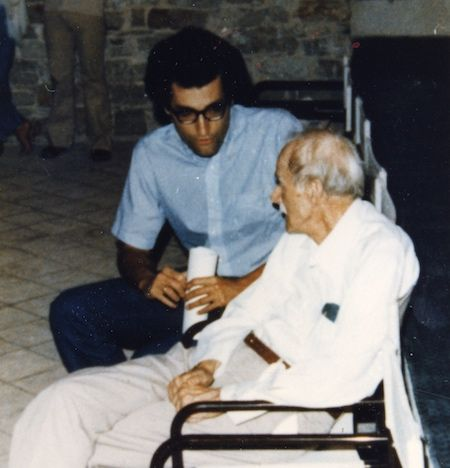
\includegraphics[width=4cm, height=4cm]{wittenDirac.jpg}\\

\noindent{}(Only If:) Assume that $R_D$ is decidable in \K{}, that is, there exists $H\in{}\bm{K}$ s.t $(H(c(A),x)=1\iff{}A(x)=b\in{}R(A)$ $\wedge{}$ $(H(c(A),x)=0\iff{}A(x)=*$. Construct $H'$ that corecognizes $R_D$ as follows: $H'=A_{sw(0,1)}\cdot{}H$ where $P_{sw(0,1)}$ switches a 0 by a 1 and is undefined for all other inputs. Hence, $H'(c(A), x)=1$ $\iff{}$ $A(x)=*$ and else $H'$ is undefined as desired.  \\

Ishaan's equation: $E=MC^2$ --- $\int_{\infty{}}^{b} x^2 \,dx$

\section{NOTING}




\end{document} 